Softare developed by ARK. \cite{bib:artesian:url}

Stores temporal series.

Esistono \texttt{Timeseries} e \texttt{Timeseries versionate}. Di queste ultime e` presente piu` di una versione per lo stesso giorno.

Retrieves data from several providers, performs ETL, exposes timeseries (retrievable via Excel or API).

Usato perche` effettua operazioni non banali sui dati che risultano comode (e sarebbe stato necessario rieffetturarle nella DWH).

\paragraph{Providers}
    \begin{itemize}
    \item MK (52602 curves)
        \begin{itemize}
            \item Temperature
            \item Consumption
            \item Wind Power
            \item Residual Load
            \item Photovoltaic
            \item Spot Price
            \item Weather
            \item Exchange
            \item Hydrology
            \item Power
        \end{itemize}
    \item Entsog (49263 curves)
        \begin{itemize}
            \item Gas Transport
            \item Interruptions
        \end{itemize}
    \item GME (1990 curves)
        \begin{itemize}
            \item Commodities
                \begin{itemize}
                    \item Power
                    \item Gas
                \end{itemize}
            \item Markets
                \begin{itemize}
                    \item MGP
                    \item MI
                    \item MSD
                        \begin{itemize}
                            \item MSD ex-ante
                            \item MB
                        \end{itemize}
                \end{itemize}
        \end{itemize}
    \item Jao (1690 curves)
        \begin{itemize}
            \item Example curves:
                \begin{itemize}
                    \item DE-FR-M-BASE\_01\_RequestCapacity
                    \item DE-FR-M-BASE\_01\_OfferedCapacity
                    \item DE-FR-M-BASE\_01\_AllocatedCapacity
                    \item DE-FR-M-BASE\_01\_ATC
                    \item DE-FR-M-BASE\_01\_Price
                    \item DE-FR-M-BASE\_01\_Resale
                    \item DE-FR-M-BASE\_01\_Maintenance
                \end{itemize}
            \item \hl{Bidding?}
            \item stock market energy
        \end{itemize}
    \item PointConnect (1495 curves)
        \begin{itemize}
            \item Power
            \item Gas
        \end{itemize}
    \item Terna\footnote{98\% RTN} (1195 curves)
        \begin{itemize}
            \item Power (ITA)
        \end{itemize}
    \item EEX\footnote{European Energy Exchange} (1147 curves)
        \begin{itemize}
            \item Power (companies, fuel)
        \end{itemize}
    \item Jao\_Axpo (817 curves)
        \begin{itemize}
            \item Bidding
            \item dati privati
        \end{itemize}
    \item SNAM (671 curves)
        \begin{itemize}
            \item dati privati
            \item Gas
                \begin{itemize}
                    \item Stoccaggio
                    \item Esportazioni
                    \item immesso
                    \item riconsegnato
                    \item roba sul bilanciamento
                \end{itemize}
            \item Temperature
                \begin{itemize}
                    \item temperature rilevate (massima e minima per citta`)
                \end{itemize}
            \item GNL\footnote{Liquefied Natural Gas}
                \begin{itemize}
                    \item scaricato
                    \item immesso
                    \item allocato
                    \item stoccaggio
                    \item 
                \end{itemize}
            \item Trasporti su gas, gnl
        \end{itemize}
    \item TPO (598 curves)
        \begin{itemize}
            \item da pfx11 interni
            \item PowerPlants
            \item Power
        \end{itemize}
    \item Genscape\footnote{Azienda che ha piazzato sensori davanti a centrali, riporta dati live sulle produzioni} (482 curves)
        \begin{itemize}
            \item Power centrali
        \end{itemize}
    \item Renen (374 curves)
        \begin{itemize}
            \item Electricity fonti rinnovabili (ITA)
        \end{itemize}
    \item \hl{OPP} (234 curves)
        \begin{itemize}
            \item 
        \end{itemize}
    \item ENEL (216 curves)
        \begin{itemize}
            \item Power
            \item indisponibilita`
        \end{itemize}
    \item \hl{BiddingUC\_Sources} (204 curves)
        \begin{itemize}
            \item 
        \end{itemize}
    \item \hl{BiddingUC\_User} (204 curves)
        \begin{itemize}
            \item 
        \end{itemize}
    \item TrayportAssessmentEngine (162 curves)
        \begin{itemize}
            \item Open/High/Low/Close
            \item Power
            \item Gas
            \item Coal
        \end{itemize}
    \item ENI (43 curves)
        \begin{itemize}
            \item Power
            \item Indisponibilita`
        \end{itemize}
    \item Edison (28 curves)
        \begin{itemize}
            \item Power
            \item Indisponibilita`
        \end{itemize}
    \item I4c (28 curves)
        \begin{itemize}
            \item \hl{curve per bidding uc}
        \end{itemize}
    \item TERNASunSet (28 curves)
        \cite{bib:terna_sunset:url}
        \begin{itemize}
            \item contratti dispacciamento in immisione e prelievo
            \item prezzi
        \end{itemize}
    \item Alba (20 curves)
        \begin{itemize}
            \item prezzi di mercato (open/high/low/close) su
                \begin{itemize}
                    \item gas
                    \item power
                    \item co2
                    \item coal
                    \item cv
                \end{itemize}
        \end{itemize}
    \item Tirreno (19 curves)
        \begin{itemize}
            \item indisponibilita` remit
        \end{itemize}
    \item MeteoGroup (14 curves)
        \begin{itemize}
            \item fct/act per diverse centrali su
                \begin{itemize}
                    \item pressione
                    \item umidita`
                    \item temperature
                \end{itemize}
        \end{itemize}
    \item Damas (10 curves)
        \begin{itemize}
            \item Capacity auctions on Italian borders
            \item prezzo di transito da/a
                \begin{itemize}
                    \item RTE (FR)
                    \item SWG (CH\footnote{Svizzera})
                    \item APG (AU)
                    \item ELES (SI\footnote{Slovenia})
                    \item HTSO (GR)
                \end{itemize}
        \end{itemize}
    \item \hl{AxpoRTM} (4 curves)
        \begin{itemize}
            \item 
        \end{itemize}
    \item \hl{RTM} (4 curves)
        \begin{itemize}
            \item 
        \end{itemize}
    \item \hl{TRIMP} (3 curves)
        \begin{itemize}
            \item 
        \end{itemize}
    \item \hl{OG} (2 curves)
        \begin{itemize}
            \item 
        \end{itemize}
\end{itemize}

\paragraph{ETL}
    \begin{itemize}
        \item estrazione da varie fonti
        \item Aggregazione/deaggregazione dove necessario
        \item normalizzazione dati
        \item controlli nel caso di assenza di dati (si possono ricavare da informazioni aggregate diversamente, pero` ci si deve assicurare coincidano)
    \end{itemize}
    
\paragraph{Data extraction}
    Si possono estrarre dati sia tramite UI che tramite API
    
    Processo:
    \begin{itemize}
        \item selezionare curve desiderate (vedi figure \ref{fig:artesian:select_curves})
            \begin{figure}
                \centering
                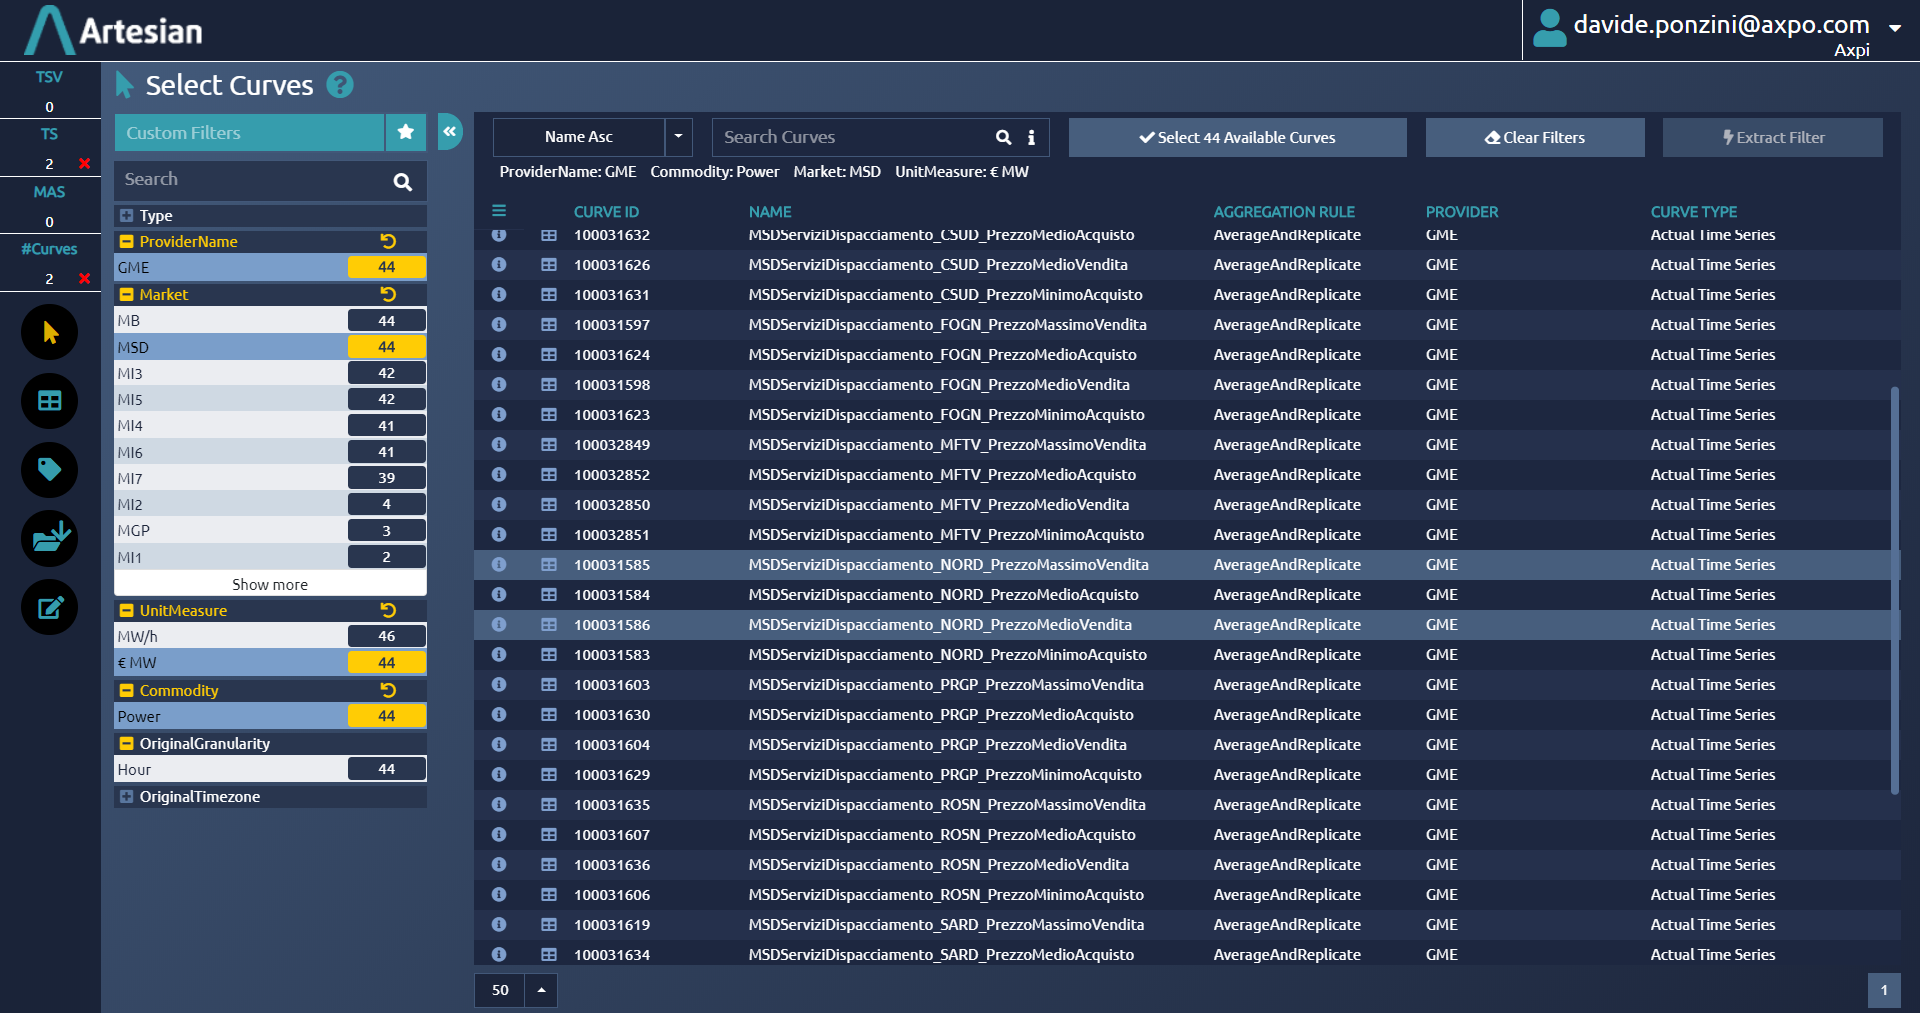
\includegraphics[width=\textwidth]{res/artesian/select_curves.png}
                \caption{Curve selection in Artesian}
                \label{fig:artesian:select_curves}
            \end{figure}
        \item pannello extract
        \item specificare date
            \begin{itemize}
                \item range
                \item relative
                    \begin{itemize}
                        \item rolling week
                        \item rolling month
                        \item rolling quarter
                        \item rolling year
                        \item week to (current) date
                        \item month to date
                    \end{itemize}
                \item period from/to
                \item period (d+1, m+3, y-1, ecc)
            \end{itemize}
        \item selezionare versione (per curve versionate)
            \begin{itemize}
                \item muv (most updated version) si prende sempre il dato piu` recente disponibile
                \item etc (non ci interessano)
            \end{itemize}
        \item selezionare granularita
            \begin{itemize}
                \item 10min to month
            \end{itemize}
        \item selezionare timezone
        \item selezionare time transformation
            \begin{itemize}
                \item gas day 6-6\footnote{Il giorno gas inizia alle 6am e finisce alle 6am del giorno dopo}
                \item thermal year\footnote{L'anno termico inizia il 1 ott e termina il 30 sett}
            \end{itemize}
    \end{itemize}
